\documentclass[12pt]{book}
\usepackage[a4paper,left=1cm,right=1cm,top=3cm,bottom=4cm,bindingoffset=5mm]{geometry}
\usepackage{fancyhdr}
%\usepackage{lscape} %für Querfromat
\usepackage{cancel} %um was in durchzustreichen
\usepackage{paralist} %um in enumerate einfach andere Sachen anzugeben
\usepackage{amsmath}
\usepackage{amssymb}
\usepackage{amsthm}
\usepackage{subcaption}
\usepackage{todonotes}
\usepackage[ngerman]{babel}
\usepackage[utf8]{inputenc}
%\usepackage{MnSymbol}
\usepackage{mathabx} % damit man Doppelklammern haben kann
\setlength{\parindent}{0em}  %verhindert Einrücken nach Absatz
\usepackage{xargs} %
\usepackage{tikz} %zum zeichnen
\usepackage{expdlist} % um den Zeilenabstand in description kleiner zu machen


\newcommand\tab[1][1cm]{\hspace*{#1}}

%\setmathfont[range={\lsem,\rsem}]{XITS Math}

% Meine Schrift, die mathe kann
\usepackage[math]{iwona}
\usepackage[T1]{fontenc}


\pagestyle{fancy}
\fancyhf{}
\lhead{Graph Drawing - Layer Assignment}
\rhead{ Thomas Dost, Jonas Lange, Francesca Rybicki}

\begin{document}
 
\section*{Subject}

%We aim to visualize the \textit{Layer Assignment} phase of the \textit{Layered} layout algorithm step by step.
Unser Ziel ist es, die  \textit{Layer Assingment} Phase des \textit{Layered} layout Algorithmuses zu visualisieren. 
Hierbei gibt die Graphische Schittstelle dem Benutzer die Möglichkeit, den Algorithums Schritt für Schritt betrachtet. 
So soll  der Benutzer durch Ausprobieren ein intuitives Verständniss für den Algorithmus entwickeln. Wichtig ist uns
dabei die verständliche Visualisierung des Algorithmuses, so wie eine intuitiv zu bedienende GUI. Weniger wichtig ist
uns allerdings eine gute Performance bei sehr großen Graphen.

\todo[inline]{write summarizing stuff here, add source of layered paper}

\section*{Our Approach}

here should be some general information about things we do.

\begin{enumerate}
    \item first we parse
    \item Als nächstes wenden wir \textit{Layer Assingment} Algorithmus auf den Elkgraphen an. Hierbei erstellen wir nach
    jedem Schritt einen SimpleGraph (vereinfachte Graphenstruktur, die nur die notwendigen Informeationen für die
    Visualisierung enthällt) aus dem Elkgraphen. Nachdem der \textit{Layer Assingment} Algorithmus fertig ist, geben wir 
    eine Liste dieser SimpleGraphs an die Visualisierung weiter.
    \item then we visualize
\end{enumerate}

\todo[inline]{write general information on your topic here, e.g what is you input, what is yout output, any methods you use.. but don't go into detail yet. this will happen in your very own chapter }

\section*{Approach in detail}

\todo[inline]{write a subchapter about your topic. go into details, if there is something you really want to mention, because its cool or so.. especially try to use stuff from lecture (sources, technical terms, etc. ) if you want to give reasons for your solution. 

Further: explain the input and output formats of your special topic -> iLearn has some MUSTs listed here, be sure you considered those.}

\newpage




\subsection*{Parsing}
Die Parsing-Klasse ist dafür zuständig das eigens erstelle Textformate einzulesen
und in einen ElkGraph umzuwandeln, zusätlich wird der eingelesene Graph auf Kreisfreiheit überprüft
da der Layer-Assignment-Algorithmus nur für kreisfreie Graphen definiert ist.

\subsubsection*{Syntax}
Eine Node hinzufügen:
\newline
\tab[0.5cm]  node \_$<$node name$>$
\newline
\newline
Eine Edge hinzufügen:\newline
\tab[0.5cm]  edge\_$<$start node$>$ \_$<$end node$>$
\newline
Wobei \_ für beliebig viele Whitespaces steht,
weiter muss jeder Knoten der von einer edge benutzt wird vorher mit dem \textit{node} Keyword eingeführt werden

\subsubsection*{Methoden}
Parser.parse(<filepath>)\newline
Return: null falls ein fehler auftrat, sonst ein ElkGraph

\subsubsection*{Benutzung des Parsers}
try 
\{\newline
ElkNode testGraph = Parser.parse("testGraphs/testfile.txt");
\newline
\}
\newline
catch (Exception e)
\newline
\{
\newline
  e.printStackTrace(); 
\newline
\}


\subsubsection*{Beispiel}
node n1 \newline
node n2 \newline
node n3 \newline
\newline
\newline
edge n1 n3\newline 
edge n2 n3 \newline










\newpage
\documentclass[a4paper,10pt]{scrartcl}

\begin{document}
Die Klasse LayerAssignment enthällt eine Reihe hilfreicher Funktionen, die Wichtigste ist allerdings die Methode assignLayers. assignLayers nimmt einen ElkGraphen, führt das Layerassignment an ihm durch und gibt eine Bearbeitungshistorie in Form einer ArrayList vom typen MyGraph zurück. Wobei MyGraph eine von uns entwickelte vereinfachte Graphenstruktur ist. Jeder MyGraph in der Liste stellt also einen "snapshot" aus dem Layerassingments des Graphen dar.
Durch Seiteneffekte beinflusst die Methode auch den eingegebenen ElkGraphen, so dass er am Ende der Methode als vollständig gelayerter Graph vorliegt. Dazu haben wir jedem Knoten 3 Propertys gegeben:
 LAYER: Ein Integer wert größer oder gleich 1, der das Layer angibt, in dem sich der Knoten befindet

IS_DUMMY: Ein boolscher wert, der True ist, wenn es sich bei dem Knoten um einen von uns eingefügten Dummyknoten handelt. Zu beachten ist, dass auch Edges die Property IS_DUMMY haben.

POSITION_IN_LAYER: Gibt an, an welcher Stelle im Layer sich der Knoten befindet, diese Property muss in der Crossingminimisation optimiert werden.

Beim einfügen der Dummyknoten geht der Algorithmus wie folgt vor:
Wenn eine Kante k ein Layer übersprngt, fügen wir für jedes Layer zwischen den Layern des Startknotens von k und des Endknotens von k einen neuen Dummyknoten in dem jeweiligen Layer ein. Nun fügen wir Dummykanten so ein, dass von jedem Dummyknoten eine Dummykante zum Dummyknoten im nächsthöheren Layer führt. Desweiteren soll eine Dummykante vom höchsten Dummyknoten zum Zielknotne von k führen. Zuletzt wird noch der Zielknoten von k auf den Dummyknoten im Layer direkt über dem Startknoten von k gesetzt.

(Hier vlt zeichnung)


MyGraph ist eine vereinfachte Graphenstruktur. Sie enthällt nur eine Liste von Knoten und eine Liste von Kanten.  


\end{document}













\newpage



\subsection*{Visualize}














\section*{Schedule}


\begin{tabular}{|p{2cm}|*3{p{4.5cm}|}}
   
    \hline
    Date & Thomas & Jonas & Francesca \\
     \hline
     \hline
      18.6.18 & - & - & Window mockup (no functionality) \\
       \hline
    18.6.18 & Parsing finished (no cycle chek)& - & - \\
    \hline
     18.6.18 & - & First approach for Layer assignment & - \\
    \hline
   19.6.18 & \multicolumn{3}{|c|}{First Deadline/Demo} \\
    \hline \hline
     30.6.18 & - & - & Animations applied to LA algorithm \\
   \hline
     30.6.18 & - & Added some tests & - \\
   \hline
     30.6.18 & Cycle check & - & - \\
   \hline
   7.7.18 & \multicolumn{3}{|c|}{Complete Documentation} \\
    \hline
     9.7.18 &\multicolumn{3}{|c|}{Last Checks?} \\
     \hline
     10.7.18 &\multicolumn{3}{|c|}{Finished} \\
    
    \hline
\end{tabular}


\todo[inline]{Daten eintragen}

\newpage
\section*{Technical Details}

\todo[inline]{things like class diagrams maybe?}
\begin{figure}[h!]
    \centering
    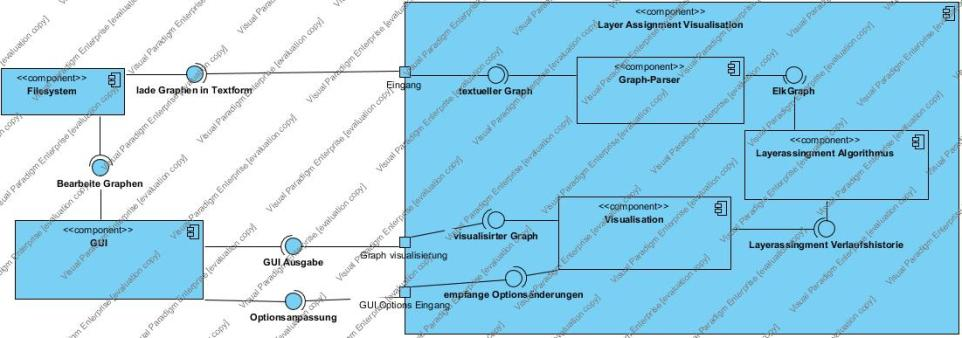
\includegraphics[width=\textwidth]{images/Component_Diagram1.jpg}
\end{figure}


\end{document}






